%----------------------------------------------------------------------------------------
% SCHAAL. Alle opgaven zijn eigen werk.
%
% Opbouw: Probleem, Start, leerstof, en op een nieuwe pagina de Opdrachten en Test jezelf (geen Koppel in de 2de graad).
% Labels van dit hoofdstuk beginnen met h1-.
% Pakketten: de homothetie met een negatieve factor staat alleen in pakket 4 en 5.
%----------------------------------------------------------------------------------------

\mychapter{1}{Schaal}

\begin{probleem}
\vspace{-1mm}\naast{Een chocolatier giet massieve paashazen van 12~cm hoog. Voor zo'n haas heeft hij 60~g chocolade nodig. Voor zijn etalage maakt hij een haas met precies dezelfde vorm, maar drie keer zo hoog: 36~cm. Hoeveel chocolade heeft hij daarvoor nodig? En hoeveel keer zoveel goudpapier om hem in te pakken? Drie keer zoveel, zou je denken. Klopt dat?}{\begin{tikzpicture}[font=\scriptsize]
  \haas{.25}{0}{.06}
  \haas{2.1}{0}{.18}
  \draw[grijs,|-|] (-.35,0) -- (-.35,.72) node[midway,left] {12};
  \draw[grijs,|-|] (3.3,0) -- (3.3,2.16) node[midway,right] {36};
\end{tikzpicture}}
\end{probleem}

\lkr{Leerplan \pakketnaam: LPD 8 (vergroten en verkleinen: lengte, oppervlakte en volume). De homothetie (sectie 2) is opgenomen omdat ze een natuurlijke ingang is voor gelijkvormigheid, en omdat GO! ze vraagt. \alleenvoor{4,5}{De negatieve factor staat alleen in pakket 4 en 5. }Voorkennis: omtrek, oppervlakte en volume van de gewone figuren en lichamen, eenheden omzetten, verhoudingen. De derdemachtswortel komt alleen voor met mooie getallen (8, 27, 64, 125, 1000).}

Een kaart, een bouwplan, een modelauto en een foto tonen iets in het klein of in het groot, maar met dezelfde vorm. In dit hoofdstuk leer je rekenen met zo'n schaal: van de tekening naar de werkelijkheid en terug. Je leert hoe je een figuur vergroot vanuit een punt, en wanneer twee figuren dezelfde vorm hebben. En je ontdekt dat oppervlaktes en volumes heel anders groeien dan lengtes. Dat verklaart waarom de grote paashaas zoveel chocolade kost.

\begin{oefeningen}[Start]
\oef{h1-start-1}

\oef{h1-verken}
\end{oefeningen}

%========================================================================================
\section{Rekenen met een schaal}

\subsection{Van de tekening naar de werkelijkheid}

Een tekening van een huis is veel kleiner dan het huis zelf. Hoe weet je dan hoe groot een kamer echt is? Neem een plattegrond waarop een kamer van 4~m lang getekend is als een rechthoek van 8~cm lang. Zet beide lengtes in dezelfde eenheid: 8~cm op het plan tegenover 400~cm in werkelijkheid. Dat is 1~cm tegenover 50~cm. Elke centimeter op het plan staat dus voor 50~cm in het echt, in elke richting. Je zegt: het plan is getekend op \emph{schaal} $\schaal{1}{50}$.

\begin{theorie}
De \textbf{\textcolor{accent}{schaal}} van een tekening is de verhouding van een lengte op de tekening tot de werkelijke lengte, in dezelfde eenheid:

\vspace{1mm}
\qquad $\formule{\text{schaal} = \text{lengte op de tekening} : \text{werkelijke lengte}}$

\vspace{1mm}
Schaal $\formule{1 : n}$ betekent: 1~cm op de tekening is $n$~cm in werkelijkheid. Bij een vergroting schrijf je de schaal als $\formule{n : 1}$.
\end{theorie}

Een schaal heeft geen eenheid. Op een kaart van $\schaal{1}{25\,000}$ is 1~cm op de kaart $25\,000$~cm in werkelijkheid, maar ook 1~mm op de kaart $25\,000$~mm. Hoe groter het getal $n$, hoe kleiner alles getekend is.

\voorbeeld{}{Op een wandelkaart met schaal $\schaal{1}{25\,000}$ liggen twee berghutten 7,4~cm uit elkaar. Hoe ver is dat in vogelvlucht?\label{vb:h1-kaart}}{%
\uitleg{Elke centimeter op de kaart is $25\,000$~cm in werkelijkheid. We vermenigvuldigen dus met $25\,000$ en zetten daarna om naar een handige eenheid.}
\begin{stappen}
7{,}4 \cdot 25\,000 = 185\,000~\text{cm} & De werkelijke lengte, in de eenheid van de kaart. \\[1ex]
185\,000~\text{cm} = 1850~\text{m} = 1{,}85~\text{km} & Deel door 100 voor meter, en nog eens door 1000 voor kilometer.
\end{stappen}
De hutten liggen 1,85~km uit elkaar. Het pad ertussen is langer, want het loopt niet recht.}

Omgekeerd deel je door $n$: een werkelijke lengte is op de tekening $n$ keer zo klein.

\voorbeeld{}{Een architect tekent een terras van 6,3~m bij 4,8~m op schaal $\schaal{1}{50}$. Hoe groot wordt de rechthoek op het plan?\label{vb:h1-plan}}{%
\uitleg{Nu gaan we van de werkelijkheid naar de tekening: we delen door 50. Zet eerst om naar centimeter, want op een plan meet je in centimeter.}
\naast{\begin{stappenvrij}{5cm}{5.2cm}
6{,}3~\text{m} = 630~\text{cm} & Omzetten naar centimeter. \\[1ex]
4{,}8~\text{m} = 480~\text{cm} & \\[1ex]
630 : 50 = 12{,}6~\text{cm} & De lengte op het plan. \\[1ex]
480 : 50 = 9{,}6~\text{cm} & De breedte op het plan.
\end{stappenvrij}}{\begin{tikzpicture}[scale=.25,font=\scriptsize]
  \filldraw[fill=accent!12,draw=accent,thick] (0,0) rectangle (12.6,9.6);
  \node[below] at (6.3,0) {12,6~cm};
  \node[right] at (12.6,4.8) {9,6~cm};
  \node at (6.3,4.8) {terras};
\end{tikzpicture}}}

\begin{werkwijze}
Zet de lengtes in dezelfde eenheid. Bij schaal $\schaal{1}{n}$ is de werkelijke lengte $n$ keer de lengte op de tekening, en de lengte op de tekening de werkelijke lengte gedeeld door $n$. Zet het resultaat om naar een eenheid die past: centimeter op een plan, meter of kilometer in het echt.
\end{werkwijze}

\nujij{Een fietsroute is op een kaart met schaal $\schaal{1}{100\,000}$ 23~cm lang. Hoe lang is ze echt?}{$23 \cdot 100\,000 = 2\,300\,000$~cm $= 23$~km.}

\begin{oefeningen}
\oef{h1-schaal}
\end{oefeningen}

\subsection{De schaal bepalen}

Op een modelauto of een foto staat de schaal niet altijd vermeld. Ken je één lengte op de tekening en dezelfde lengte in het echt, dan vind je de schaal: zet beide in dezelfde eenheid en vereenvoudig de verhouding tot $\schaal{1}{n}$ of $\schaal{n}{1}$.

\voorbeeld{}{Een modelauto is 22,5~cm lang. De echte auto is 4,05~m lang. Bepaal de schaal van het model.\label{vb:h1-bepaal}}{%
\uitleg{We zetten beide lengtes in centimeter, en delen de werkelijke lengte door die van het model: zoveel keer is het model kleiner.}
\begin{stappen}
4{,}05~\text{m} = 405~\text{cm} & Dezelfde eenheid. \\[1ex]
405 : 22{,}5 = 18 & De echte auto is 18 keer zo lang. \\[1ex]
\text{schaal } \schaal{22{,}5}{405} = \schaal{1}{18} & Deel beide getallen door 22,5.
\end{stappen}}

Bij een vergroting is de tekening groter dan de werkelijkheid. Dan deel je omgekeerd, en staat het grote getal vooraan.

\voorbeeld{}{Een lieveheersbeestje is 7~mm lang. Op een foto in een natuurboek is het 5,6~cm lang. Bepaal de schaal van de foto.\label{vb:h1-vergroting}}{%
\uitleg{De foto is groter dan het beestje: een vergroting. We zetten beide in millimeter.}
\naast{\begin{stappenvrij}{5cm}{5.2cm}
5{,}6~\text{cm} = 56~\text{mm} & Dezelfde eenheid. \\[1ex]
56 : 7 = 8 & De foto is 8 keer zo groot. \\[1ex]
\text{schaal } \schaal{8}{1} & Een vergroting: het grote getal staat vooraan.
\end{stappenvrij}}{\begin{tikzpicture}[scale=.5]
  \filldraw[fill=accent!25,draw=accent,thick] (0,0) ellipse (1.1 and .85);
  \draw[accent,thick] (0,-.85) -- (0,.85);
  \filldraw[fill=accent,draw=accent] (1.2,0) circle (.35);
  \foreach \p in {(-.5,.4),(.45,.45),(-.55,-.35),(.5,-.4)} \fill[accent] \p circle (.15);
\end{tikzpicture}}}

\nujij{Een souvenir van het Atomium is 3~cm hoog; het echte Atomium is 102~m hoog. Bepaal de schaal.}{$10\,200 : 3 = 3400$: schaal $\schaal{1}{3400}$.}

\begin{oefeningen}
\oef{h1-bepaal}
\end{oefeningen}

\subsection{De maatstok}

Vergroot je een kaart op de kopieermachine, dan klopt de schaal die erop staat niet meer: de getekende afstanden zijn langer geworden, de werkelijke niet. Daarom staat op een kaart vaak een \emph{maatstok}: een lijnstuk met de werkelijke afstand erbij. De maatstok wordt mee vergroot, dus die blijft kloppen.

\voorbeeld{}{Op de kaart hieronder hoort de maatstok van 2~cm bij 500~m. Bepaal de schaal van de kaart en de afstand in vogelvlucht van de kerk $K$ tot de molen $M$.\label{vb:h1-maatstok}}{%
\uitleg{Meet de maatstok en de afstand $KM$ met een lat. Uit de maatstok volgt de schaal, en met de schaal reken je de afstand om.}
\figuren{\begin{tikzpicture}[font=\scriptsize]
  \fill[accent!6] (-.4,-.5) rectangle (6.4,2.6);
  \draw[accent!45,line width=3pt] plot[smooth] coordinates {(-.4,1.4) (1.2,1.1) (2.6,1.6) (4,1.2) (6.4,.6)};
  \draw[grijs,dashed] (.5,.5) -- (5.3,1.9);
  \filldraw[fill=white,draw=inkt] (.35,.3) rectangle (.65,.6);
  \draw[inkt] (.5,.6) -- (.5,.95) (.4,.82) -- (.6,.82);
  \fill (.5,.5) circle (1.3pt) node[left=3pt] {$K$};
  \draw[inkt,thick] (5.3,1.9) -- ++(.3,.3) (5.3,1.9) -- ++(-.3,.3) (5.3,1.9) -- ++(.3,-.3) (5.3,1.9) -- ++(-.3,-.3);
  \fill (5.3,1.9) circle (1.3pt) node[right=5pt] {$M$};
  \maatstok{.3}{-.3}{2}{4}{500 m}
\end{tikzpicture}}
\begin{stappen}
500~\text{m} = 50\,000~\text{cm} & De maatstok: 2~cm op de kaart is $50\,000$~cm. \\[1ex]
50\,000 : 2 = 25\,000 \ \Rightarrow \ \text{schaal } \schaal{1}{25\,000} & Wat 1~cm voorstelt. \\[1ex]
\lengte{KM} = 5~\text{cm op de kaart} & Gemeten met een lat. \\[1ex]
5 \cdot 25\,000 = 125\,000~\text{cm} = 1250~\text{m} & De afstand in vogelvlucht.
\end{stappen}}

\begin{oefeningen}
\oef{h1-maatstok}
\end{oefeningen}

%========================================================================================
\section{Vergroten vanuit een punt}

\subsection{Een figuur vergroten}

Op een rooster is vergroten eenvoudig: je telt de hokjes en neemt elk lijnstuk twee keer zo lang. Maar hoe vergroot je een figuur op een wit blad, of een figuur met schuine zijden? Denk aan een lamp die de schaduw van een kartonnen driehoek op een muur werpt. Het licht vertrekt uit één punt. Elk punt van de schaduw ligt op de lichtstraal door het overeenkomstige punt van de driehoek, maar verder van de lamp. Dat idee gebruiken we om te vergroten.

\voorbeeld{}{Vergroot driehoek $ABC$ vanuit het punt $O$ met factor 2.\label{vb:h1-construeer}}{%
\uitleg{Elk punt schuift weg van $O$, langs de halfrechte vanuit $O$, tot het twee keer zo ver van $O$ ligt.}
\naast{\begin{minipage}{7.4cm}
\begin{enumerate}[leftmargin=5mm,itemsep=2pt]
\item \textit{Teken de halfrechten $[OA$, $[OB$ en $[OC$.}
\item \textit{Meet $\lengte{OA}$, en zet op $[OA$ het punt $A'$ met $\lengte{OA'} = 2 \cdot \lengte{OA}$. Doe hetzelfde voor $B'$ en $C'$.}
\item \textit{Verbind $A'$, $B'$ en $C'$.}
\end{enumerate}
\vspace{1mm}
Driehoek $A'B'C'$ is de vergroting. Elke zijde is twee keer zo lang als de overeenkomstige zijde van $ABC$, en heeft dezelfde richting.
\end{minipage}}{\begin{tikzpicture}[scale=.82,font=\scriptsize]
  \coordinate (O) at (0,0);
  \coordinate (A) at (1.5,.3); \coordinate (B) at (2.5,.9); \coordinate (C) at (1.3,1.5);
  \coordinate (A2) at (3,.6); \coordinate (B2) at (5,1.8); \coordinate (C2) at (2.6,3);
  \draw[lijngrijs] (O) -- ($(O)!1.12!(A2)$) (O) -- ($(O)!1.06!(B2)$) (O) -- ($(O)!1.08!(C2)$);
  \filldraw[fill=accent!12,draw=accent,thick] (A2) -- (B2) -- (C2) -- cycle;
  \filldraw[fill=accent!35,draw=accent,thick] (A) -- (B) -- (C) -- cycle;
  \punt[left]{0}{0}{O}
  \node[below] at (A) {$A$}; \node[above right=-2pt] at (B) {$B$}; \node[above left=-1pt] at (C) {$C$};
  \node[below] at (A2) {$A'$}; \node[right] at (B2) {$B'$}; \node[above left=-1pt] at (C2) {$C'$};
\end{tikzpicture}}}

Wat je in dit voorbeeld deed, heeft een naam. Je kunt elke figuur zo vergroten of verkleinen, met elke positieve factor.

\begin{theorie}
De \textbf{\textcolor{accent}{homothetie}} met \textbf{\textcolor{accent}{centrum}} $O$ en \textbf{\textcolor{accent}{factor}} $k$ (met $k > 0$) beeldt elk punt $P$ af op het punt $P'$ van de halfrechte $[OP$ waarvoor

\vspace{1mm}
\qquad $\formule{\lengte{OP'} = k \cdot \lengte{OP}}$

\vspace{1mm}
Het centrum is zijn eigen beeld. Voor $k > 1$ is het beeld een vergroting, voor $0 < k < 1$ een verkleining.
\end{theorie}

Een homothetie heet ook een \emph{centrische vermenigvuldiging}: je vermenigvuldigt de afstand tot het centrum met $k$. Bij $k = 1$ verandert er niets. Bij $k = \tfrac12$ schuift elk punt naar het centrum toe, tot halverwege.

\voorbeeld{}{Verklein de vierhoek $ABCD$ vanuit $O$ met factor $\tfrac12$.\label{vb:h1-verklein}}{%
\uitleg{Op een rooster hoef je niet te meten: tel hoeveel hokjes je van $O$ naar een punt gaat, naar rechts en naar boven, en neem daar de helft van.}
\naast{\begin{stappenvrij}{5.2cm}{4.6cm}
A(2, 0) \ \to \ A'(1, 0) & Vanuit $O$: 2 naar rechts wordt 1 naar rechts. \\[1ex]
B(6, 2) \ \to \ B'(3, 1) & 6 rechts en 2 omhoog wordt 3 rechts en 1 omhoog. \\[1ex]
C(4, 6) \ \to \ C'(2, 3) & Telkens de helft. \\[1ex]
D(0, 4) \ \to \ D'(0, 2) & Het centrum ligt op een rooster­punt: dat maakt tellen makkelijk.
\end{stappenvrij}}{\begin{tikzpicture}[scale=.42,font=\scriptsize]
  \ruitjes{-1}{-1}{7}{7}
  \draw[lijngrijs] (0,0) -- (2,0) (0,0) -- (6,2) (0,0) -- (4,6) (0,0) -- (0,4);
  \filldraw[fill=accent!12,draw=accent,thick] (2,0) -- (6,2) -- (4,6) -- (0,4) -- cycle;
  \filldraw[fill=accent!35,draw=accent,thick] (1,0) -- (3,1) -- (2,3) -- (0,2) -- cycle;
  \punt[below left]{0}{0}{O}
  \node[below] at (2,0) {$A$}; \node[right] at (6,2) {$B$}; \node[above] at (4,6) {$C$}; \node[left] at (0,4) {$D$};
\end{tikzpicture}}}

\begin{werkwijze}
Teken vanuit het centrum een halfrechte door elk hoekpunt. Zet op elke halfrechte het beeld, op $k$ keer de afstand tot het centrum. Op een rooster tel je de hokjes naar rechts en naar boven, en vermenigvuldig je ze met $k$. Verbind de beelden in dezelfde volgorde.
\end{werkwijze}

\begin{oefeningen}
\oef{h1-construeer}
\end{oefeningen}

\subsection{Wat blijft, en wat verandert?}

In voorbeeld~\ref{vb:h1-verklein} kun je de zijden nameten. De zijde $[AD]$ loopt van $(2, 0)$ naar $(0, 4)$, en $[A'D']$ van $(1, 0)$ naar $(0, 2)$: hetzelfde trapje, maar elke stap is half zo groot. Dus is $[A'D']$ half zo lang. Dat geldt voor elk lijnstuk.

\begin{theorie}
\begin{stelling}{Lengtes bij een homothetie}
Bij een homothetie met factor $k$ wordt elk lijnstuk $k$ keer zo lang:

\vspace{1mm}
\qquad $\formule{\lengte{A'B'} = k \cdot \lengte{AB}}$
\end{stelling}
\end{theorie}

We bewijzen dit hier niet: in het volgende hoofdstuk steunt de uitleg over gelijkvormige driehoeken er net op. Op een rooster zie je het door het trapje te tellen, en voor een figuur zonder rooster kun je het nameten. Omdat elke zijde $k$ keer zo lang wordt, wordt ook de omtrek $k$ keer zo groot.

\voorbeeld{}{Een driehoek heeft zijden van 3~cm, 4~cm en 6~cm. Hij wordt vergroot met factor 2,5. Hoe lang zijn de zijden van het beeld, en hoe groot is de omtrek van het beeld?\label{vb:h1-lengtes}}{%
\uitleg{Elke zijde wordt 2,5 keer zo lang. De omtrek kun je op twee manieren vinden.}
\begin{stappen}
3 \cdot 2{,}5 = 7{,}5, \quad 4 \cdot 2{,}5 = 10, \quad 6 \cdot 2{,}5 = 15 & De zijden van het beeld, in cm. \\[1ex]
7{,}5 + 10 + 15 = 32{,}5~\text{cm} & De omtrek van het beeld. \\[1ex]
(3 + 4 + 6) \cdot 2{,}5 = 13 \cdot 2{,}5 = 32{,}5~\text{cm} & Controle: de omtrek wordt ook 2,5 keer zo groot.
\end{stappen}}

Kijk nog eens naar de figuur van voorbeeld~\ref{vb:h1-construeer}: $[A'B']$ loopt evenwijdig met $[AB]$, en ook de andere zijden lopen evenwijdig met hun beeld. Bij het trapje in voorbeeld~\ref{vb:h1-verklein} zie je waarom: de verhouding van de stap naar boven tot de stap opzij blijft dezelfde, dus de richting ook.

\begin{theorie}
\begin{stelling}{Evenwijdig beeld}
Bij een homothetie is het beeld van een rechte een evenwijdige rechte:

\vspace{1mm}
\qquad $\formule{A'B' \parallel AB}$
\end{stelling}
\end{theorie}

Dat is handig bij het tekenen. Heb je het beeld $A'$ van één hoekpunt, dan vind je de andere beelden zonder te meten: trek door $A'$ een evenwijdige met $AB$, en waar die de halfrechte $[OB$ snijdt, ligt $B'$.

\voorbeeld{}{De homothetie met centrum $O$ beeldt $A$ af op $A'$. Teken het beeld van driehoek $ABC$ zonder te meten.\label{vb:h1-evenwijdig}}{%
\uitleg{We gebruiken dat elke zijde evenwijdig met haar beeld loopt.}
\naast{\begin{minipage}{7.4cm}
\begin{enumerate}[leftmargin=5mm,itemsep=2pt]
\item \textit{Teken de halfrechten $[OB$ en $[OC$.}
\item \textit{Trek door $A'$ de evenwijdige met $AB$. Het snijpunt met $[OB$ is $B'$.}
\item \textit{Trek door $A'$ de evenwijdige met $AC$. Het snijpunt met $[OC$ is $C'$.}
\end{enumerate}
\vspace{1mm}
Controle: $B'C'$ moet nu evenwijdig met $BC$ lopen.
\end{minipage}}{\begin{tikzpicture}[scale=.7,font=\scriptsize]
  \coordinate (O) at (0,0);
  \coordinate (A) at (1.2,-.3); \coordinate (B) at (2,1); \coordinate (C) at (.6,1.2);
  \coordinate (A2) at (3,-.75); \coordinate (B2) at (5,2.5); \coordinate (C2) at (1.5,3);
  \draw[lijngrijs] (O) -- ($(O)!1.1!(A2)$) (O) -- ($(O)!1.08!(B2)$) (O) -- ($(O)!1.1!(C2)$);
  \draw[accent,dashed] ($(A2)!-.1!(B2)$) -- ($(A2)!1.15!(B2)$) ($(A2)!-.1!(C2)$) -- ($(A2)!1.15!(C2)$);
  \draw[accent,thick] (A2) -- (B2) -- (C2) -- cycle;
  \filldraw[fill=accent!35,draw=accent,thick] (A) -- (B) -- (C) -- cycle;
  \punt[left]{0}{0}{O}
  \node[below] at (A) {$A$}; \node[right] at (B) {$B$}; \node[above left=-1pt] at (C) {$C$};
  \fill (A2) circle (1.5pt) node[below] {$A'$}; \node[right] at (B2) {$B'$}; \node[above left=-1pt] at (C2) {$C'$};
\end{tikzpicture}}}

Omdat elke zijde evenwijdig met haar beeld loopt, blijven ook de hoeken even groot: twee hoeken met evenwijdige benen in dezelfde richting zijn gelijk (denk aan de F-hoeken bij evenwijdige rechten).

\begin{theorie}
\begin{stelling}{Hoeken bij een homothetie}
Een homothetie behoudt de grootte van hoeken:

\vspace{1mm}
\qquad $\formule{\hoek{A'} = \hoek{A}}$
\end{stelling}
\end{theorie}

De lengtes veranderen dus allemaal met dezelfde factor, en de hoeken blijven gelijk. Daarom verandert de vorm niet: alleen de grootte.

\voorbeeld{}{Een driehoek $ABC$ heeft $\hoek{A} = 50^\circ$, $\hoek{B} = 60^\circ$ en $\lengte{AB} = 4$~cm. Hij wordt verkleind met factor 0,75. Wat weet je over het beeld $A'B'C'$?\label{vb:h1-hoeken}}{%
\uitleg{De hoeken blijven gelijk, de lengtes worden vermenigvuldigd met 0,75.}
\begin{stappen}
\hoek{A'} = 50^\circ, \ \hoek{B'} = 60^\circ & Een homothetie behoudt hoeken. \\[1ex]
\hoek{C'} = 180^\circ - 50^\circ - 60^\circ = 70^\circ & De hoekensom in een driehoek: zo was ook $\hoek{C} = 70^\circ$. \\[1ex]
\lengte{A'B'} = 0{,}75 \cdot 4 = 3~\text{cm} & De lengte verandert wel.
\end{stappen}}

\begin{oefeningen}
\oef{h1-blijft}
\end{oefeningen}

\begin{alleenvoor}{4,5}
\subsection{Een negatieve factor}

Wat gebeurt er als het beeld aan de andere kant van het centrum ligt? Dat zie je in een camera met een klein gaatje: de lichtstralen van een boom gaan door het gaatje en vormen achteraan een beeld dat op zijn kop staat. Het gaatje is het centrum, en het beeld ligt aan de andere kant. Dat geven we aan met een negatieve factor.

\begin{theorie}
Voor $k < 0$ beeldt de \textbf{\textcolor{accent}{homothetie}} met centrum $O$ en factor $k$ elk punt $P$ af op het punt $P'$ van de halfrechte tegenover $[OP$, met

\vspace{1mm}
\qquad $\formule{\lengte{OP'} = \abs{k} \cdot \lengte{OP}}$
\end{theorie}

Het beeld ligt dus aan de overkant van $O$, en staat op zijn kop. Lengtes worden $\abs{k}$ keer zo groot, en de hoeken blijven gelijk. Bij $k = -1$ is het beeld even groot: dat is de puntspiegeling om $O$.

\voorbeeld{}{Teken het beeld van driehoek $ABC$ bij de homothetie met centrum $O$ en factor $-\tfrac12$.\label{vb:h1-negatief}}{%
\uitleg{Het beeld ligt aan de overkant van $O$. Op het rooster tel je de hokjes van $O$ naar een punt, neem je de helft, en ga je de andere kant op.}
\naast{\begin{stappenvrij}{5cm}{4.4cm}
A(2, 2) \ \to \ A'(-1, -1) & 2 rechts en 2 omhoog wordt 1 links en 1 omlaag. \\[1ex]
B(6, 2) \ \to \ B'(-3, -1) & De helft, de andere kant op. \\[1ex]
C(4, 4) \ \to \ C'(-2, -2) & \\[1ex]
\lengte{A'B'} = 2 = \tfrac12 \cdot 4 & Lengtes met $\abs{k} = \tfrac12$.
\end{stappenvrij}}{\begin{tikzpicture}[scale=.42,font=\scriptsize]
  \ruitjes{-4}{-3}{7}{5}
  \draw[lijngrijs] (-1,-1) -- (2,2) (-3,-1) -- (6,2) (-2,-2) -- (4,4);
  \filldraw[fill=accent!12,draw=accent,thick] (2,2) -- (6,2) -- (4,4) -- cycle;
  \filldraw[fill=accent!35,draw=accent,thick] (-1,-1) -- (-3,-1) -- (-2,-2) -- cycle;
  \punt[above left]{0}{0}{O}
  \node[above left] at (2,2) {$A$}; \node[right] at (6,2) {$B$}; \node[above] at (4,4) {$C$};
  \node[above] at (-1,-1) {$A'$}; \node[left] at (-3,-1) {$B'$}; \node[below] at (-2,-2) {$C'$};
\end{tikzpicture}}}

\begin{oefeningen}
\oef{h1-negatief}
\end{oefeningen}
\end{alleenvoor}

\subsection{Gelijkvormige figuren}

Een vergroting heeft dezelfde vorm als het origineel. Schuif je het beeld daarna op, draai je het of spiegel je het, dan blijft de vorm ook dezelfde. Een foto, een kaart en een modelauto hebben zo dezelfde vorm als het echte ding, maar niet dezelfde grootte. Daar is een woord voor.

\begin{theorie}
Twee figuren zijn \textbf{\textcolor{accent}{gelijkvormig}} als de ene een vergroting of verkleining is van de andere, eventueel gevolgd door een verschuiving, een draaiing of een spiegeling. De factor $k$ heet de \textbf{\textcolor{accent}{gelijkvormigheidsfactor}}.

\begin{stelling}{Gelijkvormige veelhoeken}
Twee veelhoeken zijn gelijkvormig als hun overeenkomstige hoeken gelijk zijn en hun overeenkomstige zijden dezelfde verhouding hebben:

\vspace{1mm}
\qquad $\formule{\dfrac{\lengte{A'B'}}{\lengte{AB}} = \dfrac{\lengte{B'C'}}{\lengte{BC}} = \dfrac{\lengte{C'D'}}{\lengte{CD}} = \ldots = k}$
\end{stelling}
\end{theorie}

Een schaaltekening is zo gelijkvormig met de werkelijkheid, met als factor de schaal: bij schaal $\schaal{1}{50}$ is $k = \tfrac{1}{50}$ van de werkelijkheid naar de tekening.

\voorbeeld{}{Zijn de rechthoeken $R_1$ (4 bij 6), $R_2$ (6 bij 9) en $R_3$ (6 bij 8) gelijkvormig?\label{vb:h1-rechthoeken}}{%
\uitleg{Alle hoeken van een rechthoek zijn recht, dus de hoeken zijn telkens gelijk. We vergelijken de verhouding van de korte zijden en die van de lange zijden.}
\naast{\begin{stappenvrij}{5.2cm}{3.6cm}
R_1 \text{ en } R_2: \ \dfrac64 = 1{,}5 \text{ en } \dfrac96 = 1{,}5 & Dezelfde verhouding: gelijkvormig, $k = 1{,}5$. \\[2ex]
R_1 \text{ en } R_3: \ \dfrac64 = 1{,}5 \text{ en } \dfrac86 \approx 1{,}33 & Niet dezelfde verhouding: niet gelijkvormig.
\end{stappenvrij}}{\begin{tikzpicture}[scale=.25,font=\scriptsize]
  \ruitjes{0}{0}{19}{9}
  \filldraw[fill=accent!35,draw=accent,thick] (0,0) rectangle (4,6);
  \filldraw[fill=accent!20,draw=accent,thick] (5,0) rectangle (11,9);
  \filldraw[fill=accent!8,draw=accent,thick] (12,0) rectangle (18,8);
  \node at (2,3) {$R_1$}; \node at (8,4.5) {$R_2$}; \node at (15,4) {$R_3$};
\end{tikzpicture}}
Kijk naar de figuur: $R_3$ is in verhouding iets breder dan $R_1$, en dat zie je.}

Je hebt beide voorwaarden nodig, de hoeken en de zijden. Een vierkant en een rechthoek van 2 bij 4 hebben dezelfde hoeken, maar ze zijn niet gelijkvormig. Een vierkant en een ruit met dezelfde zijde hebben dezelfde zijden, maar andere hoeken.

\figuren{\begin{tikzpicture}[scale=.5,font=\scriptsize]
  \filldraw[fill=accent!20,draw=accent,thick] (0,0) rectangle (2,2);
  \filldraw[fill=accent!20,draw=accent,thick] (3,0) rectangle (7,2);
  \node[below] at (3.5,-.2) {dezelfde hoeken, niet gelijkvormig};
  \begin{scope}[xshift=10cm]
  \filldraw[fill=accent!20,draw=accent,thick] (0,0) rectangle (2,2);
  \filldraw[fill=accent!20,draw=accent,thick] (3,0) -- (5,0) -- ({5+2*cos(55)},{2*sin(55)}) -- ({3+2*cos(55)},{2*sin(55)}) -- cycle;
  \node[below] at (3,-.2) {dezelfde zijden, niet gelijkvormig};
  \end{scope}
\end{tikzpicture}}

\nujij{Is een driehoek met zijden 5, 7 en 8 gelijkvormig met een driehoek met zijden 10, 14 en 17?}{Nee: $\tfrac{10}{5} = \tfrac{14}{7} = 2$, maar $\tfrac{17}{8} \neq 2$.}

\begin{oefeningen}
\oef{h1-gelijkvormig}
\end{oefeningen}

%========================================================================================
\section{Oppervlakte}

\subsection{Factor \texorpdfstring{$k$}{k} voor lengtes, \texorpdfstring{$k^2$}{k²} voor oppervlaktes}

In de Verken werd de oppervlakte van de figuur vier keer zo groot toen je alle lengtes verdubbelde, en niet twee keer. Is dat toeval? Neem een rechthoek van 3 bij 2 en vergroot hem met factor 3. Het beeld is 9 bij 6. In de figuur zie je dat de grote rechthoek uit $3 \cdot 3 = 9$ kopieën van de kleine bestaat: drie in de breedte en drie in de hoogte.

\naast{De lengte en de breedte worden allebei 3 keer zo groot, dus de oppervlakte $3 \cdot 3 = 9$ keer:
\[ 9 \cdot 6 = (3 \cdot 3) \cdot (3 \cdot 2) = 3^2 \cdot (3 \cdot 2) . \]
Bij een driehoek gaat het net zo: de basis en de hoogte worden allebei $k$ keer zo lang, dus
\[ \frac{(k\,b) \cdot (k\,h)}{2} = k^2 \cdot \frac{b \cdot h}{2} . \]
En bij een cirkel wordt de straal $k$ keer zo groot: $\pi\,(k\,r)^2 = k^2 \cdot \pi r^2$.}{\begin{tikzpicture}[scale=.36,font=\scriptsize]
  \ruitjes{0}{0}{9}{6}
  \fill[accent!35] (0,0) rectangle (3,2);
  \draw[accent,thick] (0,0) rectangle (9,6);
  \draw[accent] (3,0) -- (3,6) (6,0) -- (6,6) (0,2) -- (9,2) (0,4) -- (9,4);
  \node[below] at (4.5,0) {9};
  \node[right] at (9,3) {6};
  \node at (1.5,1) {$A$};
\end{tikzpicture}}

Telkens komt er een factor $k \cdot k = k^2$ bij, omdat een oppervlakte het product is van twee lengtes.

\begin{theorie}
\begin{stelling}{Oppervlakte bij vergroten}
Wordt een figuur vergroot of verkleind met factor $k$, dan wordt haar oppervlakte $k^2$ keer zo groot:

\vspace{1mm}
\qquad $\formule{A' = k^2 \cdot A}$
\end{stelling}
\end{theorie}

Dat geldt voor elke figuur, ook voor een figuur zonder formule, zoals een meer op een kaart. Leg er een fijn rooster over en tel de hokjes: bij het vergroten wordt elk hokje een vierkant met een $k$ keer zo lange zijde, dus met een $k^2$ keer zo grote oppervlakte. Een veel gemaakte fout is de oppervlakte met $k$ vermenigvuldigen in plaats van met $k^2$.

\voorbeeld{}{Op een kaart met schaal $\schaal{1}{5000}$ heeft een park een oppervlakte van 6~cm$^2$. Hoe groot is het park echt?\label{vb:h1-opp}}{%
\uitleg{Van de kaart naar de werkelijkheid is de factor $k = 5000$. Een oppervlakte wordt dus met $5000^2$ vermenigvuldigd, niet met 5000.}
\begin{stappen}
k^2 = 5000^2 = 25\,000\,000 & De factor voor oppervlaktes. \\[1ex]
6 \cdot 25\,000\,000 = 150\,000\,000~\text{cm}^2 & De werkelijke oppervlakte. \\[1ex]
150\,000\,000 : 10\,000 = 15\,000~\text{m}^2 & Want $1~\text{m}^2 = 100 \cdot 100~\text{cm}^2 = 10\,000~\text{cm}^2$.
\end{stappen}
Het park is $15\,000$~m$^2$ groot, of 1,5~ha. Wie met 5000 vermenigvuldigt, vindt $30\,000$~cm$^2$ = 3~m$^2$: kleiner dan een slaapkamer.}

\nujij{Een tekening op schaal $\schaal{1}{20}$ van een tafelblad heeft een oppervlakte van 45~cm$^2$. Hoe groot is het tafelblad?}{$45 \cdot 400 = 18\,000$~cm$^2$ $= 1{,}8$~m$^2$.}

\subsection{Van oppervlakte terug naar lengte}

Soms ken je de factor voor de oppervlakte en zoek je de factor voor de lengtes. Dan werk je omgekeerd: $k^2$ is gegeven, dus $k$ is de vierkantswortel.

\voorbeeld{}{Een blad A3 is gelijkvormig met een blad A4 en heeft een dubbel zo grote oppervlakte. Een A4 is 21~cm bij 29,7~cm. Met welke factor vergroot een kopieermachine van A4 naar A3, en hoe groot is een A3?\label{vb:h1-a4}}{%
\uitleg{De oppervlakte wordt 2 keer zo groot, dus $k^2 = 2$. De factor voor de lengtes is dan $\sqrt2$.}
\naast{\begin{stappenvrij}{5cm}{4.4cm}
k^2 = 2 \ \Rightarrow \ k = \sqrt2 \approx 1{,}41 & Een kopieermachine toont daarom 141~\%. \\[1ex]
21 \cdot \sqrt2 \approx 29{,}7~\text{cm} & De korte zijde van A3: de lange van A4. \\[1ex]
29{,}7 \cdot \sqrt2 \approx 42{,}0~\text{cm} & De lange zijde van A3.
\end{stappenvrij}}{\begin{tikzpicture}[scale=.07,font=\scriptsize]
  \filldraw[fill=accent!12,draw=accent,thick] (0,0) rectangle (29.7,42);
  \draw[accent,dashed] (0,21) -- (29.7,21);
  \filldraw[fill=accent!35,draw=accent,thick] (34,0) rectangle (55,29.7);
  \node at (14.85,10.5) {A4}; \node at (14.85,31.5) {A4};
  \node[above] at (14.85,42) {A3};
  \node[above] at (44.5,29.7) {A4};
\end{tikzpicture}}
Een A3 is 29,7~cm bij 42,0~cm. Je ziet in de figuur dat er precies twee A4's in passen, gekanteld.}

\begin{werkwijze}
Bepaal de factor $k$ voor de lengtes, uit de schaal of uit twee overeenkomstige lengtes. Vermenigvuldig een oppervlakte met $k^2$. Ken je omgekeerd de factor voor de oppervlakte, neem dan de vierkantswortel: dat is $k$.
\end{werkwijze}

\begin{oefeningen}
\oef{h1-opp}
\end{oefeningen}

%========================================================================================
\section{Volume}

\subsection{Factor \texorpdfstring{$k^3$}{k³} voor volumes}

Nu kunnen we terug naar de paashaas. Hij wordt drie keer zo hoog, maar ook drie keer zo breed en drie keer zo dik. Hoeveel keer zo groot wordt zijn volume? Begin met een eenvoudiger lichaam: een kubus. Verdubbel je de ribbe, dan passen er in de grote kubus 2 kubusjes in de breedte, 2 in de hoogte en 2 in de diepte: $2 \cdot 2 \cdot 2 = 8$ kubusjes.

\figuren{\begin{tikzpicture}[schuin,scale=.6,font=\scriptsize]
  \blokje{0}{0}{0}
  \node[below] at (.5,0,0) {ribbe 1};
  \begin{scope}[xshift=3cm]
  \foreach \z in {1,0}{\foreach \y in {0,1}{\foreach \x in {0,1}{\blokje{\x}{\y}{\z}}}}
  \node[below] at (1,0,0) {ribbe 2: 8 kubusjes};
  \end{scope}
  \begin{scope}[xshift=7.2cm]
  \foreach \z in {2,1,0}{\foreach \y in {0,1,2}{\foreach \x in {0,1,2}{\blokje{\x}{\y}{\z}}}}
  \node[below] at (1.5,0,0) {ribbe 3: 27 kubusjes};
  \end{scope}
\end{tikzpicture}}

Een volume is het product van drie lengtes: de lengte, de breedte en de hoogte. Elke lengte wordt $k$ keer zo groot, dus het volume $k \cdot k \cdot k = k^3$ keer. Een balk van 1 bij 2 bij 3 heeft volume 6; met factor 2 wordt hij 2 bij 4 bij 6, met volume $48 = 8 \cdot 6$.

\begin{theorie}
\begin{stelling}{Volume bij vergroten}
Wordt een lichaam vergroot of verkleind met factor $k$, dan wordt zijn volume $k^3$ keer zo groot:

\vspace{1mm}
\qquad $\formule{V' = k^3 \cdot V}$
\end{stelling}
\end{theorie}

Net als bij de oppervlakte geldt dat voor elk lichaam, ook voor een paashaas: denk hem opgebouwd uit heel kleine kubusjes. Is het lichaam massief en van hetzelfde materiaal, dan wordt ook de massa $k^3$ keer zo groot. Zijn oppervlakte, zoals de verf of het papier errond, wordt maar $k^2$ keer zo groot.

\voorbeeld{}{Een maquette van een sporthal op schaal $\schaal{1}{200}$ heeft een volume van 900~cm$^3$. Hoe groot is het volume van de echte sporthal?\label{vb:h1-vol}}{%
\uitleg{Van de maquette naar de werkelijkheid is $k = 200$. Het volume wordt met $200^3$ vermenigvuldigd.}
\begin{stappen}
k^3 = 200^3 = 8\,000\,000 & De factor voor volumes. \\[1ex]
900 \cdot 8\,000\,000 = 7\,200\,000\,000~\text{cm}^3 & Het werkelijke volume. \\[1ex]
7\,200\,000\,000 : 1\,000\,000 = 7200~\text{m}^3 & Want $1~\text{m}^3 = 100^3~\text{cm}^3 = 1\,000\,000~\text{cm}^3$.
\end{stappen}}

Nu kunnen we het probleem oplossen.

\voorbeeld{}{Terug naar het probleem. Een paashaas van 12~cm hoog kost 60~g chocolade. Hoeveel chocolade kost een haas met dezelfde vorm van 36~cm hoog, en hoeveel keer zoveel goudpapier?\label{vb:h1-terug}}{%
\uitleg{De grote haas is een vergroting van de kleine. Eerst zoeken we de factor $k$. De hoeveelheid chocolade hangt af van het volume, het papier van de oppervlakte.}
\naast{\begin{stappenvrij}{5.4cm}{4.6cm}
k = \dfrac{36}{12} = 3 & De factor voor de lengtes. \\[2ex]
k^3 = 27 \ \Rightarrow \ 27 \cdot 60 = 1620~\text{g} & De chocolade: een volume. \\[1ex]
k^2 = 9 & Het goudpapier: een oppervlakte.
\end{stappenvrij}}{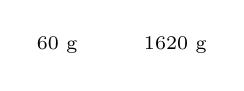
\begin{tikzpicture}[font=\scriptsize]
  \haas{.2}{0}{.05}
  \haas{1.7}{0}{.15}
  \node[below] at (.2,0) {60 g};
  \node[below] at (1.7,0) {1620 g};
\end{tikzpicture}}
De grote haas kost 1620~g chocolade, ruim anderhalve kilo: niet 3 maar 27 keer zoveel. Hij heeft 9 keer zoveel goudpapier nodig.}

Zo is het probleem opgelost, en het antwoord is verrassend. Een haas die maar drie keer zo hoog is, kost 27 keer zoveel chocolade. Daarom zijn grote chocoladefiguren bijna altijd hol.

\subsection{Van volume terug naar lengte}

Ken je de factor voor het volume, dan zoek je een getal dat tot de derde macht die factor geeft: de \emph{derdemachtswortel}. Met mooie getallen vind je die uit het hoofd: $2^3 = 8$, $3^3 = 27$, $4^3 = 64$, $5^3 = 125$ en $10^3 = 1000$. Op een rekenmachine heeft de derdemachtswortel een eigen toets.

\voorbeeld{}{Twee vazen zijn gelijkvormig. In de kleine past 0,5~liter, in de grote 4~liter. De kleine is 15~cm hoog. Hoe hoog is de grote?\label{vb:h1-terugvol}}{%
\uitleg{De inhoud is een volume. De grote vaas bevat 8 keer zoveel, dus $k^3 = 8$.}
\begin{stappen}
k^3 = \dfrac{4}{0{,}5} = 8 & De factor voor het volume. \\[2ex]
k = 2 & Want $2^3 = 8$. \\[1ex]
2 \cdot 15 = 30~\text{cm} & De hoogte is een lengte.
\end{stappen}
De grote vaas is maar twee keer zo hoog, maar bevat acht keer zoveel.}

\begin{werkwijze}
Bepaal de factor $k$ voor de lengtes. Lengtes en omtrekken vermenigvuldig je met $k$, oppervlaktes met $k^2$, volumes en massa's met $k^3$. Ken je de factor voor het volume, dan is $k$ de derdemachtswortel ervan.
\end{werkwijze}

\needspace{9\baselineskip}
Een overzicht, met als voorbeeld een vergroting met factor 3:

\begin{center}\arrayrulecolor{accent}\renewcommand{\arraystretch}{1.5}%
\begin{tabular}{|>{\centering\arraybackslash}m{3.6cm}|>{\centering\arraybackslash}m{2.6cm}|>{\centering\arraybackslash}m{3.6cm}|}
\hline
\textbf{grootheid} & \textbf{factor} & \textbf{bij $k = 3$} \\ \hline
lengte, omtrek & $k$ & 3 \\ \hline
oppervlakte & $k^2$ & 9 \\ \hline
volume, massa & $k^3$ & 27 \\ \hline
hoek & 1 & blijft gelijk \\ \hline
\end{tabular}
\end{center}

\nujij{Een kubusvormige doos met ribbe 10~cm bevat 1~liter. Hoeveel bevat een kubusvormige doos met ribbe 30~cm?}{$k = 3$, $k^3 = 27$: 27~liter.}

\begin{oefeningen}
\oef{h1-vol}
\end{oefeningen}

%========================================================================================
\opdrachtenkop

\begin{oefeningen}
\oef{h1-o1}

\oef{h1-o2}

\oef{h1-o3}

\oef{h1-o4}

\oef{h1-o5}

\oef{h1-o6}

\oef{h1-o7}

\oef{h1-o8}

\oef{h1-o9}

\oef{h1-o10}

\oef{h1-o11}

\oef{h1-o12}

\oef{h1-o13}

\oef{h1-o14}

\oef{h1-o15}

\oef{h1-o16}

\oef{h1-o17}

\oef{h1-o18}

\oef{h1-o19}

\oef{h1-o20}

\oef{h1-o21}

\oef{h1-o22}

\oef{h1-o23}

\oef{h1-o24}
\end{oefeningen}

%----------------------------------------------------------------------------------------
\opdrachtsectie{Test jezelf}

\begin{oefeningen}
\oef{h1-t1}

\oef{h1-t2}

\oef{h1-t3}

\oef{h1-t4}

\oef{h1-t5}

\oef{h1-t6}

\oef{h1-t7}
\end{oefeningen}

\herhaalschema{%
  \fv{oef:h1-t1}{vb:h1-kaart}{oef:h1-schaal}%
  \fv{oef:h1-t2}{vb:h1-bepaal}{oef:h1-bepaal}%
  \fv{oef:h1-t3}{vb:h1-verklein}{oef:h1-construeer}%
  \fv{oef:h1-t4}{vb:h1-rechthoeken}{oef:h1-gelijkvormig}%
  \fv{oef:h1-t5}{vb:h1-opp}{oef:h1-opp}%
  \fv{oef:h1-t6}{vb:h1-vol}{oef:h1-vol}%
  \fv{oef:h1-t7}{vb:h1-terugvol}{oef:h1-o19}}

\ifzelfstudie
\section*{Maak je eigen samenvatting}
Sluit dit boek en schrijf in je schrift: wat een schaal $\schaal{1}{n}$ betekent en hoe je ermee rekent, wat een homothetie is en hoe je een figuur vergroot vanuit een punt, wat er bij een homothetie gebeurt met lengtes, richtingen en hoeken, wanneer twee figuren gelijkvormig zijn, en met welke factor een lengte, een oppervlakte en een volume vermenigvuldigd worden. Vergelijk daarna met de kaders.
\fi
